


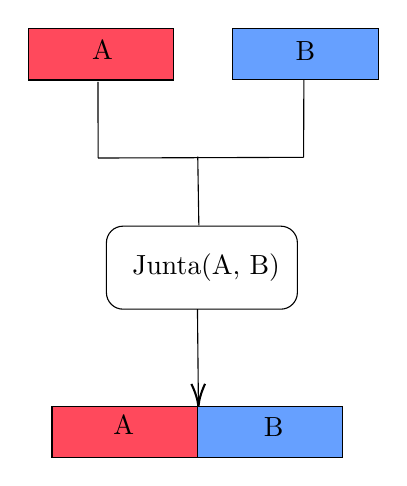
\begin{tikzpicture}[x=0.75pt,y=0.75pt,yscale=-1,xscale=1]
%uncomment if require: \path (0,300); %set diagram left start at 0, and has height of 300

%Shape: Circle [id:dp2700581997395959] 
%\draw  [fill={rgb, 255:red, 255; green, 202; blue, 64 }  ,fill opacity=1 ] (194.36,330.07) .. controls (194.36,323.85) and (199.41,318.8) .. (205.63,318.8) .. controls (211.85,318.8) and (216.89,323.85) .. (216.89,330.07) .. controls (216.89,336.29) and (211.85,341.33) .. (205.63,341.33) .. controls (199.41,341.33) and (194.36,336.29) .. (194.36,330.07) -- cycle ;
%Rounded Rect [id:dp17006798515443122] 
\draw   (364.67,131.66) .. controls (364.67,127.24) and (368.25,123.66) .. (372.67,123.66) -- (448.67,123.66) .. controls (453.08,123.66) and (456.67,127.24) .. (456.67,131.66) -- (456.67,155.66) .. controls (456.67,160.08) and (453.08,163.66) .. (448.67,163.66) -- (372.67,163.66) .. controls (368.25,163.66) and (364.67,160.08) .. (364.67,155.66) -- cycle ;
%Straight Lines [id:da9040270232690516] 
\draw    (408.67,90.17) -- (409.2,123.3) ;
%Straight Lines [id:da5000031479986659] 
\draw    (408.53,163.63) -- (408.98,208.6) ;
\draw [shift={(409,210.6)}, rotate = 269.43] [color={rgb, 255:red, 0; green, 0; blue, 0 }  ][line width=0.75]    (10.93,-3.29) .. controls (6.95,-1.4) and (3.31,-0.3) .. (0,0) .. controls (3.31,0.3) and (6.95,1.4) .. (10.93,3.29)   ;
%Straight Lines [id:da04489765783849464] 
\draw    (360.67,90.83) -- (459.67,90.5) ;
%Straight Lines [id:da19669995521828676] 
\draw    (360.6,54.2) -- (360.67,90.83) ;
%Straight Lines [id:da638670025967639] 
\draw    (459.8,52.6) -- (459.67,90.5) ;
%Shape: Rectangle [id:dp9336815212866543] 
\draw  [fill={rgb, 255:red, 255; green, 73; blue, 92 }  ,fill opacity=1 ] (327,28.5) -- (397,28.5) -- (397,53.25) -- (327,53.25) -- cycle ;
%Shape: Rectangle [id:dp4996871048748288] 
\draw  [fill={rgb, 255:red, 102; green, 160; blue, 255 }  ,fill opacity=1 ] (425.6,28.3) -- (495.6,28.3) -- (495.6,53.05) -- (425.6,53.05) -- cycle ;
%Shape: Rectangle [id:dp5861288763432269] 
\draw  [fill={rgb, 255:red, 255; green, 73; blue, 92 }  ,fill opacity=1 ] (338.44,210.42) -- (408.44,210.42) -- (408.44,235.17) -- (338.44,235.17) -- cycle ;
%Shape: Rectangle [id:dp3848827559612372] 
\draw  [fill={rgb, 255:red, 102; green, 160; blue, 255 }  ,fill opacity=1 ] (408.44,210.42) -- (478.44,210.42) -- (478.44,235.17) -- (408.44,235.17) -- cycle ;

% Text Node
\draw (356.48,33.19) node [anchor=north west][inner sep=0.75pt]   [align=left] {A};
% Text Node
\draw (454.58,33.45) node [anchor=north west][inner sep=0.75pt]   [align=left] {B};
% Text Node
\draw (375.91,135.9) node [anchor=north west][inner sep=0.75pt]   [align=left] {Junta(A, B)};
% Text Node
\draw (366.8,213.88) node [anchor=north west][inner sep=0.75pt]   [align=left] {A};
% Text Node
\draw (439.32,214.43) node [anchor=north west][inner sep=0.75pt]   [align=left] {B};


\end{tikzpicture}

